\section{Problem Setups}
Due to the inherent limitations of current computing systems, 
obtaining sufficiently precise solutions is both computationally expensive and time-consuming. 
These challenges arise from the constraints imposed by the clock speed of computing units, 
as described by 
Moore's Law \cite{Moore_Law}, 
as well as the relatively low communication speeds between these units. 
While modern numerical methods have advanced to a level where they can produce 
satisfactory results within acceptable time frames across many research domains, 
the increasing scale of problems we aim to solve has driven the search for more 
cost-effective approaches. This has led to a growing interest in neural networks as a promising alternative.

In this project, I aim to evaluate the performance of the Finite-Difference Time-Domain (FDTD) 
method and the Physics-Informed Neural Network (PINN) model within parallelized computing 
environments by find the steady-state solution of PDEs.
These two methodologies broadly represent the current approaches to 
handling PDEs, specifically 
CPU-based parallelization and GPU-based parallelization.

\subsection{General Form}
Starting with the general form of the PDEs, rather than the specific euqations, is because 
different equations give perform differently on the same compute system.
To this end, consider the previously discussed form of PDEs shown in 
equation \ref{EQ_General_PDEs} which parametrized by number $\lambda$ and an operator $\mathcal{N}[\cdot; \lambda]$.
Moreover, we assume the variable $x$ is a 2D or 3D spatio vector which is written in 
$\vec{x} \in \mathbb{R}^d$, $d = 2, 3$.
\begin{align}\label{EQ_General_Form_PDE}
  &\frac{\partial u}{\partial t}\left(t,\vec{x}\right) + \mathcal{N}\left[u(t,\vec{x});\lambda\right] = 0, &\vec{x}\in\Omega, &t\in[0, +\infty) \nonumber\\
  &u\left(0,\vec{x}\right) = \varphi (\vec{x}), &\vec{x}\in\Omega & \\
  &u\left(t,\vec{x}\right) = g (t,\vec{x}),     &\vec{x}\in \overline{\Omega}, &t\in[0, +\infty) \nonumber
\end{align}
The domain of this PDE system is considered between $0$ and $1$, where is denoted with $\Omega = [0, 1]^d$, $d = 2,3$.
To these setups, we have the general form of the PDEs we are going to investigated, shown in equations \ref{EQ_General_Form_PDE}
The boundary condition shown in E.q. \ref{EQ_General_Form_PDE} is Dirichlet Condition known as first type boundary condition, where as the 
second type boundary condition (Von Neumman) [E.q. \ref{EQ_Von_Neumman_BC}] gives the other form of $u(t,\vec{x})$ at the boundary $\overline{\Omega}$.
\begin{equation}\label{EQ_Von_Neumman_BC}
  \frac{\partial u}{\partial \vec{x}} = g(t, \vec{x}),\:\: \vec{x}\in \overline{\Omega}, \:\:t\in[0, +\infty)
\end{equation}


\subsection{Computiational Topology}
The computational topology is critically important when we are programming parallel PDEs solver softwares.
Put the strongly speed-dependent data into the slow memory could make entire program slower.

\paragraph{Callan}
The cluster we are using for this project is \texttt{Callan} \cite{Callan_TCD} which has 
$2$ CPUs per compute node, and each CPU has $32$ cores with single thread. 
The Non-Uniform Memory Access (NUMA) nodes are layout as following 
\begin{figure}[htbp]
  \centering
  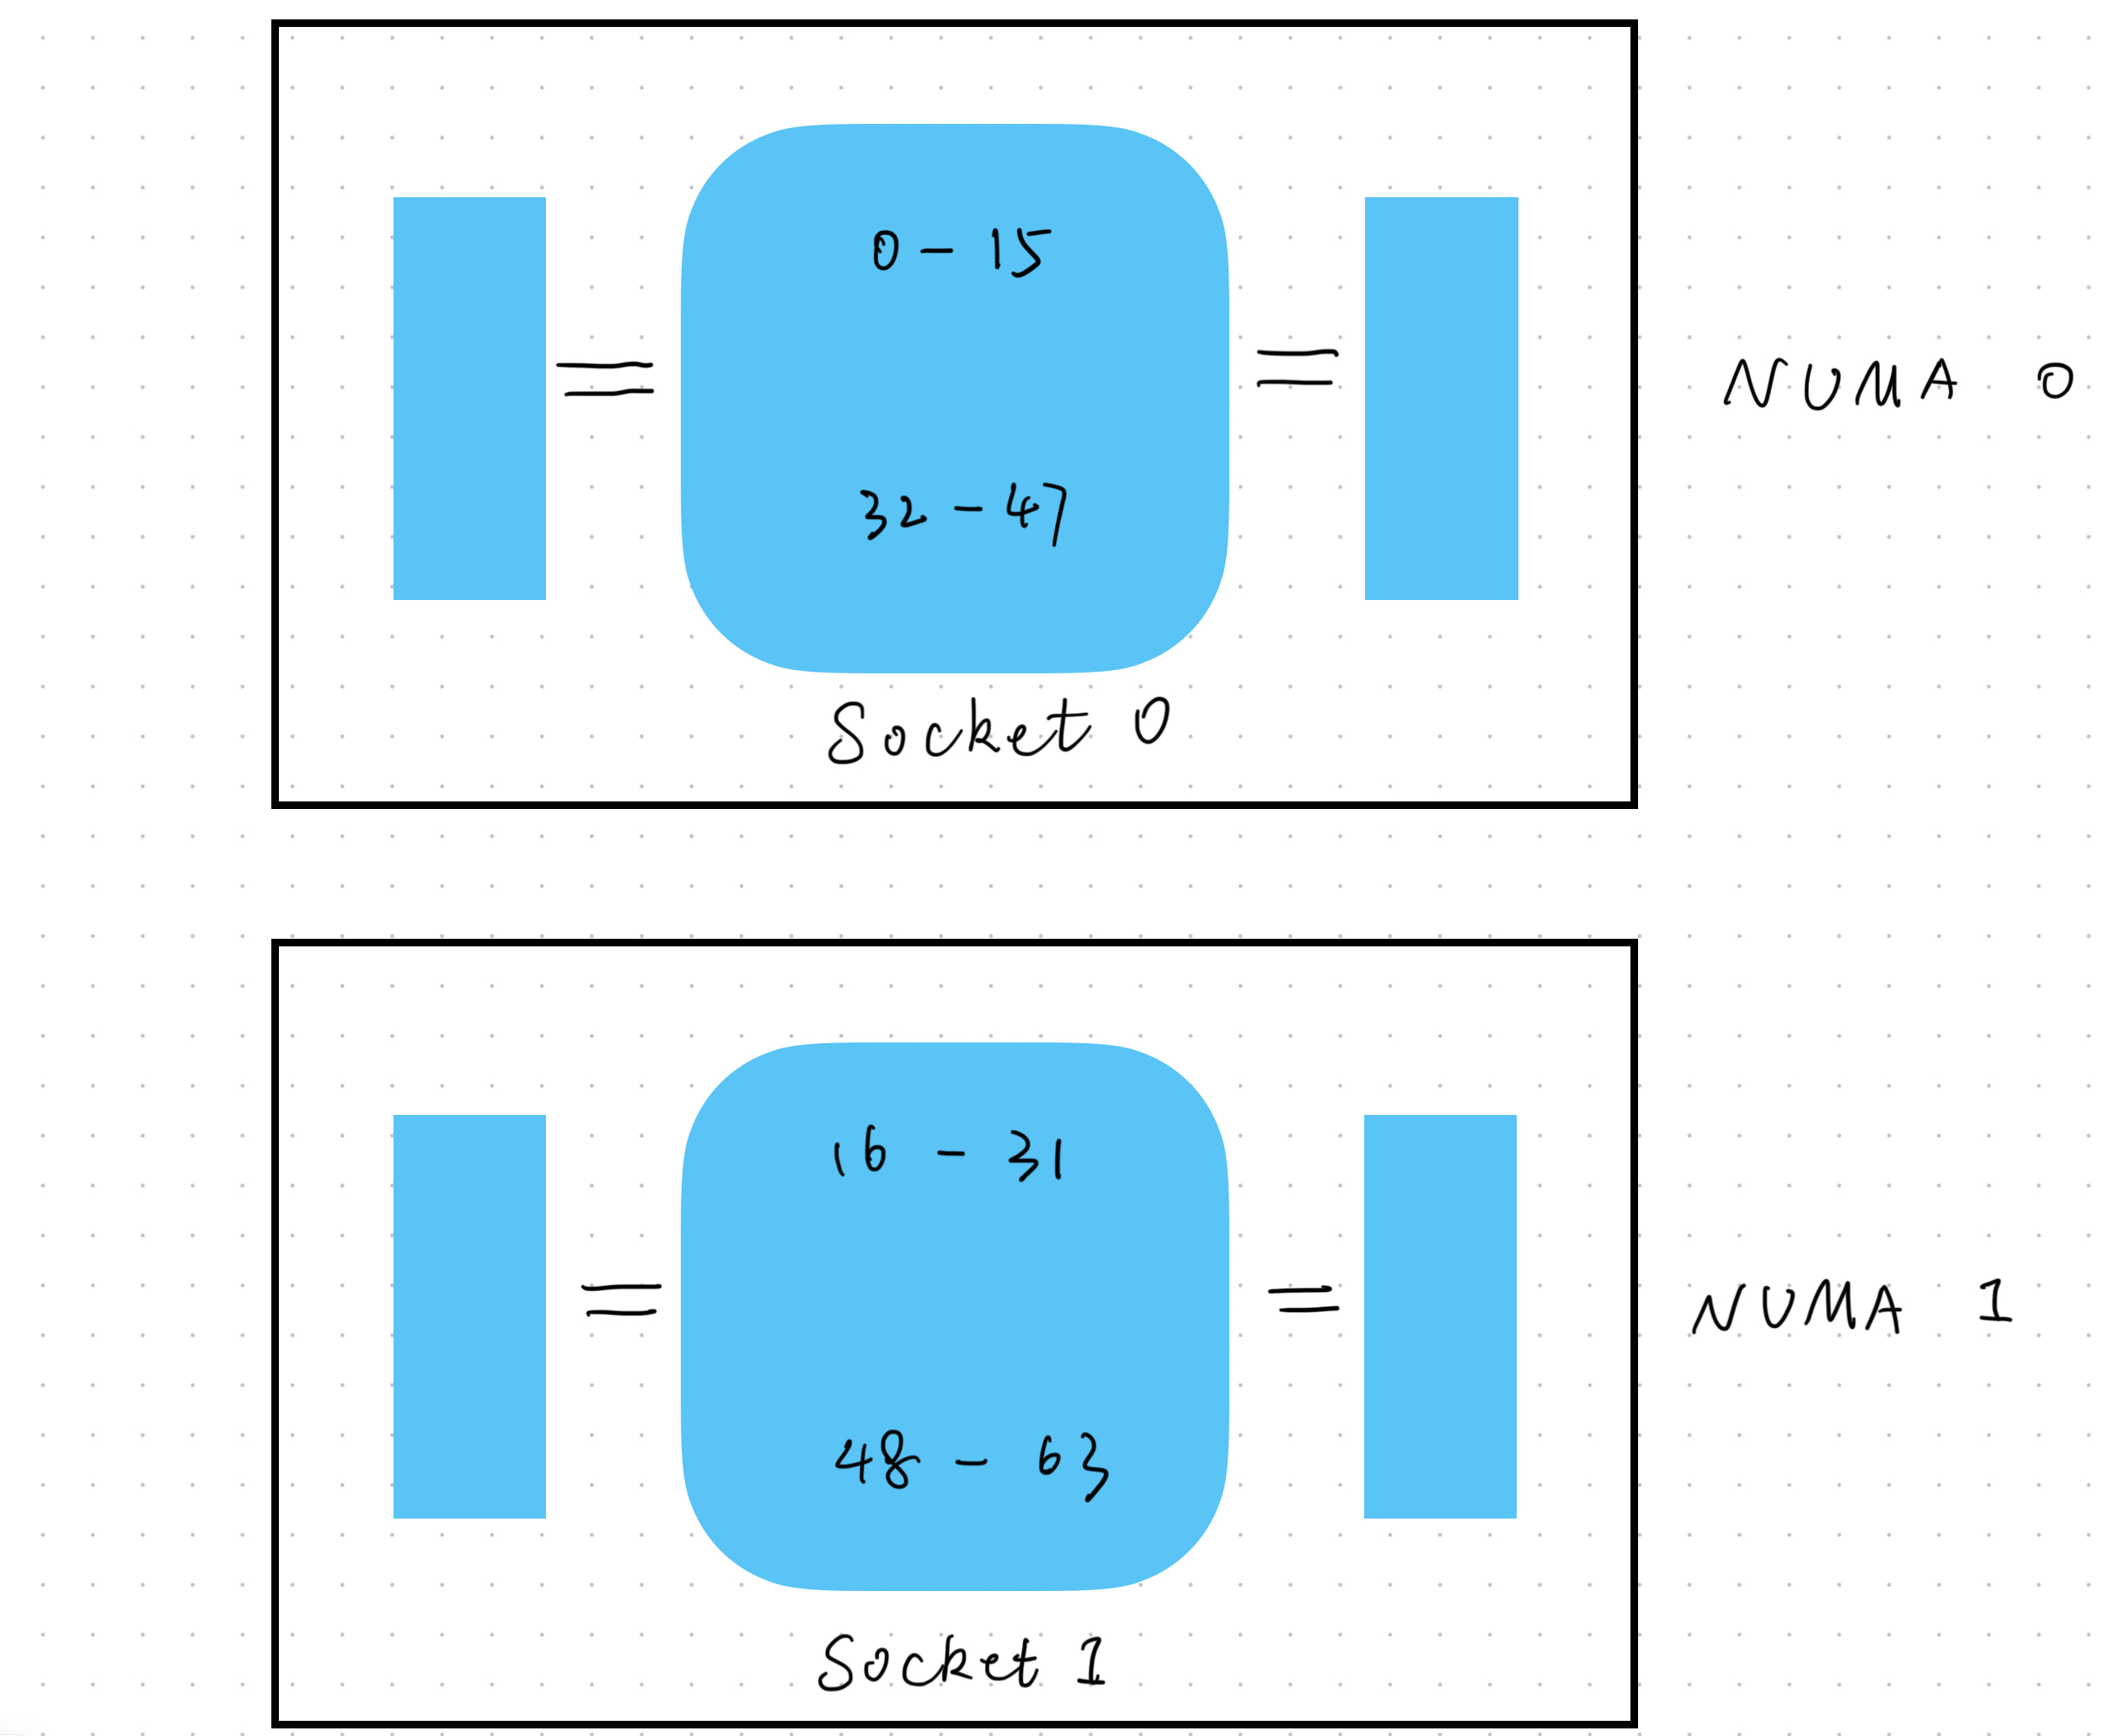
\includegraphics[width=0.5\textwidth]{figure/FIG_Topology_Callan.jpg}
  \caption{NUMA topology of single node on Callan}
  \label{FIG_Topology_Callan}
\end{figure}
Accessing the other NUMA node's memory reduces the bandwidth and also the latency,
though the bandwidth is commonly high enough, the latency can increase by 
$~30\%$ to $~400\%$ \cite{NUMA_Latency_TCD}. 
This latency becomes dangerous when writing shared memory parallel programs.


\subsection{Accuracy}
When we tried to represent numbers using arithmetic in binary, decimal or hexadecimal, truncation always affects the precision of every number, 
or so called as 
round-off-error.

\subsubsection{Round-off Error}
In IEEE-754 \cite{IEEE_754} standards, a $32$-bit floating pointer number, single precision, obligatorily represented with $23$-bit mantissa, 
$8$-bit exponent and $1$-bit for sign. 
Where as $64$-bit floating number, double precision, also ubiquitous used, which has $11$-bit exponent and $52$-bit mantissa.
After almost three decades development, not only single and double precisions (float32, float64) are ubiquitously in use, 
also more formats such as fp4, fp8, and fp16 etc. Both of them follows the simple form of exponent $k$, sign $n$ and mantissa $N$. 
\cite{IEEE_754_p2_eq1}
\begin{equation*}
  2^{k+1-N}n
\end{equation*}
Round-off errors are a manifestation of the fact that on a digital computer, which is unavoidable in numerical computations.
In such case, the precision of the number depends on how many bytes are used to store single number. 
For instance, a float32 number provides $2^{-23} \approx 1.2\times10^{-7}$, and a double precision number gives $2^{-53} \approx 2.2\times10^{-16}$, 
such number is called machine $\epsilon$ which is the smallest number the machine can represent with given format.

In numerical methods I investigated, the FDTDs are conventionally using double precision number so that the programs can treat extreamly large and small 
numbers simultaneously in the same computation, without worring about the round-off errors.
However, as mentioned, fp32 and fp16 are also popular use in scientific computing, especially in machine learning training process. 
While the lasted training GPUs are integrated compute accelarate unit for low precision floating numbers. \cite{NVIDIA_HB200_PAPER}.

\subsubsection{Floating-point Arithmetic}
The other type loss comes from the arithmetic operations on two numbers $x$, $y$. 
The standard model holds that 
\begin{equation}
  fl(x \:\text{op}\: y) = (x \: \text{op} \: y) (1+\delta), \:\:\: \left|\delta\right| < \epsilon
\end{equation}
where the op stands for the four elementary operations: $+, -, \times, /$. \cite{Germund,NMSC,V1,P112}.
